\chapter{Limits of direct reinforcement learning of decision tree policies}\label{sec:pomdp}

From the previous chapter, we know that to directly learn decision tree policies that optimize the RL objective (cf. definition~\ref{def:mdp-obj}) for an MDP (cf. definition~\ref{def:mdp}), one can learn a deterministic partially observable policy that optimizes the interpretable RL objective (cf. definition~\ref{def:irl}) in an IBMDP (cf. definition~\ref{def:ibmdp} and proposition~\ref{def:po-policy}).
Such problems are classical instances of partially observable Markov decision processes (POMDPs)~\cite{POMDP,chap2}.
This connection with POMDPs brings novel insights to direct reinforcement learning of decision tree policies. 
In this chapter, all the decision processes have a finite number of vector-valued states and observations.
Hence we will use bold fonts for states and observations but we can still use summations rather than integrals when required.

\section{Partially observable iterative Markov decision processes}\label{sec:poibmdp}
A POMDP is an MDP where the current state is hidden; only some information about the current state is observable.

\begin{definition}[Partially observable Markov decision process]\label{def:pomdp}
A partially observable Markov decision process is a tuple $\langle X, A, O, R, T, T_0, \Omega\rangle$ where:
\begin{itemize}
    \item $X$ is the hidden state space.
    \item $A$ is a finite set of actions.
    \item $O$ is a set of observations.
    \item $T: X \times A \rightarrow \Delta(X)$ is the transition function, where $T(\boldsymbol{x}_t, a, \boldsymbol{x}_{t+1}) = P(\boldsymbol{x}_t|\boldsymbol{x}_{t+1}, a)$ is the probability of transitioning to state $\boldsymbol{x}_{t}$ when taking action $a$ in state $\boldsymbol{x}$
    \item $T_0$: is the initial distribution over states. 
    \item $\Omega: X \rightarrow \Delta(O)$ is the observation function, where $\Omega(\boldsymbol{o}, a, \boldsymbol{x}) = P(\boldsymbol{o}|\boldsymbol{x}, a)$ is the probability of observing $\boldsymbol{o}$ in state $\boldsymbol{x}$
    \item $R: X \times A \rightarrow \mathbb{R}$ is the reward function, where $R(\boldsymbol{x}, a)$ is the immediate reward for taking action $a$ in state $\boldsymbol{x}$
\end{itemize}
Note that $\langle X, A, R, T, T_0 \rangle$ defines an MDP.
\end{definition}

Let us define explicitly a partially observable iterative bounding Markov decision process (POIBMDP). It is essentially an IBMDP for which we explicitly define an observation space and an observation function:
\begin{definition}[Partially observable iterative bounding Markov decision process]\label{def:poibmdp} a partially observable iterative bounding Markov decision process $\mathcal{M}_{POIB}$ is a tuple:
    \begin{align*}
        \langle \overbrace{S\times O}^{\text{States}}, \underbrace{A\cup A_{info}}_{Action space},\overbrace{O}_{\text{Observations}} ,\underbrace{(R, \zeta)}^{Rewards}, \overbrace{(T_{info}, T, T_0)}_{Transitions}, \Omega \rangle
    \end{align*}
    , where $\langle S\times O, A\cup A_{info}, (R, \zeta),( T, T_0, T_{info})\rangle$ is an IBMDP (cf. definition~\ref{def:ibmdp}).
    The transition function $\Omega$ maps concatenation of state features and observations--IBMDP states--to observations, $\Omega:S\times O \rightarrow O$, with $P(\boldsymbol{o}|(\boldsymbol{s}, \boldsymbol{o}))=1$ 
\end{definition}

One can see POIBMDPs as particular instances of POMDPs where the observation function simply applies a mask over some features of the hidden state.
This setting has other names in the literature.
For example, POIBMDPs are mixed observability MDPs \cite{momdp} with base MDP state features as the \textit{hidden variables} and feature bounds as \textit{visible} variables.
POIBMDPs can also be seen as non-stationary MDPs (N-MDPs)~\cite{learning-pomdp} in which there is one different transition function per base MDP state: these are called hidden-mode MDPs~\cite{hmmdp}.
Following~\cite{learning-pomdp} we can write the value of a deterministic partially observable policy $\pi:O\rightarrow A\cup A_{info}$ in observation $\boldsymbol{o}$.

\begin{definition}[Partially observable value function]\label{def:vpo} In a POIBMDP (cf. definition~\ref{def:poibmdp}), the expected cumulative discounted reward of a deterministic partially observable policy $\pi:O\rightarrow A\cup A_{info}$ starting from observation $o$ is $V^{\pi}(\boldsymbol{o})$:
    \begin{align*}
        V^{\pi}(\boldsymbol{o}) &= \underset{(s,\boldsymbol{o}')\in S\times O}{\sum}P^{\pi}((\boldsymbol{s}, \boldsymbol{o}')|\boldsymbol{o})V^{\pi}((\boldsymbol{s}, \boldsymbol{o}'))
    \end{align*}
with $P^{\pi}((\boldsymbol{s}, \boldsymbol{o}')|\boldsymbol{o})$ the asymptotic occupancy distribution (see \cite[section 4]{learning-pomdp} for the full definition) of the hidden POIBMDP state $(\boldsymbol{s},\boldsymbol{o}')$ given the partial observation $o$ and $V^{\pi}((s, o'))$ the classical state-value function (cf. definition~\ref{def:vs}).
We abuse notation and denote both values of observations and values of states by $V$ since the function input is not ambiguous.
\end{definition}

The asymptotic occupancy distribution is the probability of a policy $\pi$ to arrive in $(s,\boldsymbol{o}')$ while observing $\boldsymbol{o}$ in some trajectory.  
In this chapter, we use reinforcement learning to train decision tree policies for MDPs by seeking deterministic partially observable policies that optimize the interpretable RL objective (cf. definition~\ref{def:irl}) in POIBMDPs (cf. definition~\ref{def:poibmdp}).
% We summarized the approach in figure~\ref{fig:summary-rl}  

% \begin{figure}
% \centering
% \begin{tikzpicture}
%     \draw[fill=blue!40] (0, 0) rectangle (6, 4);
%     \node at (3, 3.5) {POIBMDP $\mathcal{M}_{POIB}\langle\mathcal{M}_{IB}, O, \Omega\rangle$};
%     \draw[fill=blue!30] (0, 0) rectangle (5.9, 3);
%     \node at (3, 2.5) {IBMDP $\mathcal{M}_{IB} \langle \mathcal{M}, A_{info}, \zeta \rangle$};
%     \draw[fill=blue!10] (0, 0) rectangle (5, 2);
%     \node at (3, 1.5) {MDP $\mathcal{M} \langle S, A, R, T, T_0 \rangle$};
    
%     \draw[fill=red!10] (10, 0) rectangle (14, 3);
%     \node at (12, 2) {\textbf{Objective~\ref{def:irl}}};
%     \node at (12, 1) {$\pi^{\star} = \underset{\pi}{\operatorname{argmax}} V^{\pi}(\boldsymbol{o}_0)$};
    
%     \draw[fill=red!10] (1, -5) rectangle (5, -2);
%     \node at (3, -3) {\textbf{Decision Tree Policy}};
%     \node at (3, -4) {$\pi_{\mathcal{T}}: S \rightarrow A$};
    
%     \draw[fill=red!10] (9.5, -5) rectangle (14.5, -2);
%     \node at (12, -3) {\textbf{Deterministic policy}};
%     \node at (12, -4) {$\pi: O \rightarrow A \cup A_{info}$};
    
%     \draw[thick, ->] (6, 2) -- (10, 2) node[midway, above] {$\gamma$};
%     \draw[thick, <-] (5, -3.5) -- (9.5, -3.5) node[midway, above] {Extract tree with algorithm\ref{alg:extract-tree}};
%     \draw[thick, ->] (12, 0) -- (12, -2) node[midway, left] {Solve with e.g. RL~\ref{sec:rl}};
%     \draw[thick, <-] (3, 0.5) -- (3, -2) node[midway, left] {Can be interpreted};

    
%     % % Final arrow from tree back to base MDP - adjusted position
%     % \draw[thick, ->] (1.75, -2.5) -- (1.75, -0.5) node[midway, right] {Can deploy\\and interpret};
    
% \end{tikzpicture}
% \caption{A formal framework to learn decision tree policies for MDPs that directly optimize a trade-off between the RL objective~\ref{def:mdp-obj} and interpretability.
% This framework relies on learning a deterministic partially observable policy in a POIBMDP~\ref{def:poibmdp}.}
% \label{fig:summary-rl}
% \end{figure}
The goal of the following sections is to see if, unlike indirect approaches tested in section~\ref{sec:limits-il} (cf. figures~\ref{fig:objectives} and~\ref{fig:ql-il}), direct approaches can consistently learn the depth-1 decision tree policies that have good interpretability-performance trade-offs for the $2\times 2$ grid world from example~\ref{example:grid} (cf. figures~\ref{fig:trees-intro} and~\ref{fig:optimal-policy-trees}).
The direct approach optimizes the interpretable RL objective~\ref{def:irl} in POIBMDPs (cf. definition~\ref{def:poibmdp}).
We will use reinforcement learning to learn deterministic partially observable policies for the IBMDP from example~\ref{example:ibmdp} re-written as a POIBMDP.
Next we show how to choose $\gamma$ and $\zeta$ in the POIBMDP such that the optimal deterministic partially observable policies w.r.t. the interpretable RL objective correspond exactly to the depth-1 decision tree policies with good interpretability-performance trade-offs.
Hence, if we find that RL can consistently find optimal policies w.r.t. interpretable RL objective, it means that this direct approach can consistently find the depth-1 decision tree policies with good interpretability-performance trade-off that indirect approaches could not consistently find.

\section{Constructing POIBMDPs whose optimal solutions are depth-1 decision tree policies}\label{sec:opt-depth1}
\begin{figure}
    \centering
    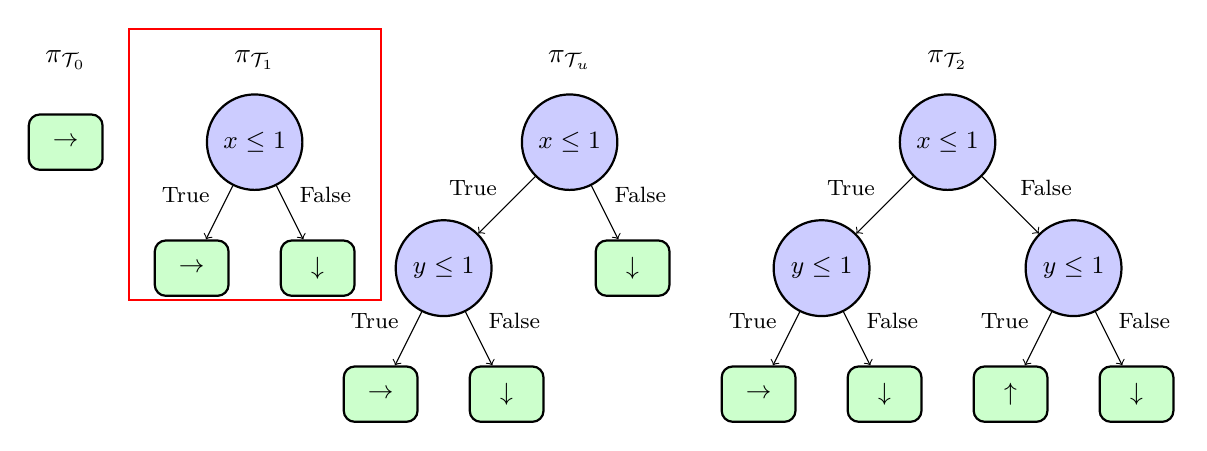
\begin{tikzpicture}[
        scale=0.8,
        decision/.style={circle, draw, thick, fill=blue!20, text width=2.5em, text centered, minimum height=2.5em, font=\small},
        leaf/.style={rectangle, draw, thick, fill=green!20, text width=2em, text centered, rounded corners, minimum height=2em, font=\small},
        edge_label/.style={font=\footnotesize, midway}
    ]
        
        \node[leaf] at (-3, 0) {$\rightarrow$};
        % Tree 4: if x <= 0.5 move right else move left
        \node[decision] (tree4_root) at (0,0) {$x \leq 1$};
        \node[leaf] (tree4_right) at (-1,-2) {$\rightarrow$};
        \node[leaf] (tree4_left) at (1,-2) {$\downarrow$};
        \draw[->] (tree4_root) -- (tree4_right) node[edge_label, above left] {True};
        \draw[->] (tree4_root) -- (tree4_left) node[edge_label, above right] {False};
        
        % Draw a square around the tree
        \draw[thick, red] (-2, 1.8) rectangle (2, -2.5);

        % Tree 7: if x <= 0.5 and y <= 0.5 move right else move down
        \node[decision] (tree7_root) at (5,0) {$x \leq 1$};
        \node[decision] (tree7_y) at (3,-2) {$y \leq 1$};
        \node[leaf] (tree7_right) at (2,-4) {$\rightarrow$};
        \node[leaf] (tree7_down) at (4,-4) {$\downarrow$};
        \node[leaf] (tree7_down2) at (6,-2) {$\downarrow$};
        \draw[->] (tree7_root) -- (tree7_y) node[edge_label, above left] {True};
        \draw[->] (tree7_root) -- (tree7_down2) node[edge_label, above right] {False};
        \draw[->] (tree7_y) -- (tree7_right) node[edge_label, above left] {True};
        \draw[->] (tree7_y) -- (tree7_down) node[edge_label, above right] {False};


        \node[decision] (tree7_root) at (11,0) {$x \leq 1$};
        \node[decision] (tree7_y) at (9,-2) {$y \leq 1$};
        \node[decision] (tree7_y2) at (13,-2) {$y \leq 1$};
        \node[leaf] (tree7_right) at (8,-4) {$\rightarrow$};
        \node[leaf] (tree7_down) at (10,-4) {$\downarrow$};
        \node[leaf] (tree7_right2) at (12,-4) {$\uparrow$};
        \node[leaf] (tree7_down2) at (14,-4) {$\downarrow$};
        \draw[->] (tree7_root) -- (tree7_y) node[edge_label, above left] {True};
        \draw[->] (tree7_root) -- (tree7_y2) node[edge_label, above right] {False};
        \draw[->] (tree7_y) -- (tree7_right) node[edge_label, above left] {True};
        \draw[->] (tree7_y) -- (tree7_down) node[edge_label, above right] {False};
        \draw[->] (tree7_y2) -- (tree7_right2) node[edge_label, above left] {True};
        \draw[->] (tree7_y2) -- (tree7_down2) node[edge_label, above right] {False};

        % Labels
        \node[above] at (-3,1) {$\pi_{\mathcal{T}_0}$};
        \node[above] at (0,1) {$\pi_{\mathcal{T}_1}$};
        \node[above] at (5,1) {$\pi_{\mathcal{T}_u}$};
        \node[above] at (11,1) {$\pi_{\mathcal{T}_2}$};


    \end{tikzpicture}
    \caption{For each decision tree structure, e.g., depth-1 or unbalanced depth-2, we illustrate a decision tree which maximizes the RL objective (cf. definition~\ref{def:mdp-obj}) in the grid world MDP.}
    \label{fig:optimal-policy-trees}
\end{figure}

Because we know all the base states, all the observations, all the actions, all the rewards and all the transitions of our POIBMDP (cf. example~\ref{example:ibmdp}), we can compute exactly the values of different deterministic partially observable policies given, $\zeta$ the reward for IGAs, and $\gamma$ the discount factor.
Each of those policies can be one of the trees illustrated in figure~\ref{fig:optimal-policy-trees}: 

\begin{itemize}
    \item $\pi_{\mathcal{T}_0}$: a depth-0 tree equivalent to always taking the same base action 
    \item $\pi_{\mathcal{T}_1}$: a depth-1 tree equivalent alternating between an IGA and a base action 
    \item $\pi_{\mathcal{T}_u}$: an unbalanced depth-2 tree that sometimes takes two IGAs then a base action and sometimes a an IGA then a base action
    \item $\pi_{\mathcal{T}_2}$: a depth-2 tree that alternates between taking two IGAs and a base action
    \item an infinite ``tree'' that only takes IGAs
\end{itemize}
Furthermore, because from~\cite{learning-pomdp} we know that for POMDPs, stochastic partially observable policies can sometimes get better expected discounted rewards than deterministic partially observable policies, we also compute the value of the stochastic policy that randomly alternates between two base actions: $\rightarrow$ and $\downarrow$.
Those two base actions always lead to the goal state (cf. figure~\ref{example:grid}).

\begin{proposition}[Depth-1 decision tree objective value] The interpretable RL objective value (cf. definition~\ref{def:irl}) of depth-1 decision tree policies with good interpretability–performance trade-offs in the grid world MDP (cf. figures~\ref{fig:trees-intro} and~\ref{fig:optimal-policy-trees}) is $\frac{4\zeta + \gamma + 2\gamma^3 + \gamma^5}{4(1-\gamma^2)}$.
\end{proposition}

We defer the lengthy proofs of this proposition, as well as the interpretable RL objective values of other decision tree policies, to the appendix~\ref{calcs}.

\begin{figure}
    \centering
    \includegraphics[width=0.6\textwidth]{images/images_part1/objective_values_plot.pdf}
    \caption{Interpretable RL objective values (cf. definition~\ref{def:irl}) of different partially observable policies as functions of $\zeta$. Shaded areas show the optimal \textit{deterministic} partially observable policies in different ranges of $\zeta$ values.}\label{fig:irl-objectives}
\end{figure}

We can now plot, in figure~\ref{fig:irl-objectives}, the interpretable RL objective values of the different partially observable policies as functions of $\zeta$ when we fix $\gamma=0.99$. 
When $\gamma=0.99$, despite objective values being very similar for the depth-1 and unbalanced depth-2 tree, we now know from the green shaded area that a depth-1 tree is the optimal one, w.r.t. the interpretable RL objective, deterministic partially observable POIBMDP policy for $0< \zeta < 1$.

Let us now define a POIBMDP with the grid world (cf. figure~\ref{example:grid}) as the base MDP, with IGAs as in the IBMDP from example~\ref{example:ibmdp}, with $\gamma=0.99$ and $0<\zeta<1$ and verify if RL can learn the optimal deterministic partially observable policies w.r.t. the interpretable RL objective, which are equivalent to depth-1 decision tree policies, in this very controlled experiment.

\section{Reinforcement learning in PO(IB)MDPs}

In general, the policy that maximizes the RL objective (cf. definition~\ref{def:mdp-obj}) in a POMDP (cf. definition~\ref{def:pomdp}) maps ``belief states'' or observation histories~\cite{chap2} to actions. Hence, those policies are not solutions to our problem since we require that policies depend only on the current observation.
If we did not have this constraint, we could apply any standard RL algorithm to solve POIBMDPs by seeking such policies because both histories and belief states are sufficient statistics for POMDP hidden states~\cite{chap2,lambrechts2025informed}.

In particular, the problem of finding the optimal deterministic partially observable policies for POMDPs is NP-HARD, even with full knowledge of transitions and rewards~\cite[section 3.2]{littman1}.
It means that it is impractical to enumerate all possible policies and take the best one. 
For even moderate-sized POMDPs, a brute-force approach would take a very long time since there are $|A|^{|O|}$ deterministic partially observable policies.
Hence it is interesting to study reinforcement learning for finding the best deterministic partially observable policy since it would not search the whole solution space.
However applying RL to our interpretable RL objective (cf. definition~\ref{def:irl}) is non-trivial.

In~\cite[Fact 2]{learning-pomdp}, the authors show that the optimal partially observable policy can be stochastic. Hence, policy gradient algorithms~\cite{pg_sutton}--that return stochastic policies--are to avoid since we seek the best \textit{deterministic} policy. 
Furthermore, the optimal deterministic partially observable policy might not maximize all the values of all observations simultaneously ~\cite[Fact 5]{learning-pomdp} which makes it difficult to use TD-learning (cf. algorithms~\ref{alg:qlearning} and~\ref{alg:sarsa}).
Indeed, doing a TD-learning update of one partially observable value (cf. definition~\ref{def:vpo}) with, e.g. Q-learning, can change the value of \textit{all} other observations in an uncontrollable manner because of the dependence in $P^{\pi}((s, \boldsymbol{o}')|\boldsymbol{o})$ (cf. definition~\ref{def:vpo}).
Interestingly, those two challenges of learning in POMDPs described in \cite{learning-pomdp} are visible in figure~\ref{fig:irl-objectives}. 
First, there is a whole range of $\zeta$ values for which the optimal partially observable policy is stochastic.
Second, for e.g. $\zeta=0.5$, while a depth-1 tree is the optimal deterministic partially observable policy, the value of state $(\boldsymbol{s}_2, \boldsymbol{o}_0) = (1.5, 1.5, 0, 2, 0, 2)$ is not maximized by this partially observable policy but by the sub-optimal policy that always goes down.

Despite those hardness results, empirical results of applying RL to POMDPs by naively replacing $\boldsymbol{x}$ by $\boldsymbol{o}$ in Q-learning or Sarsa, has already demonstrated successful in practice~\cite{sarsa-pomdp}. 
More recently, the framework of Baisero et. al. called asymmetric RL~\cite{baisero-dqn,baisero-ppo} has also shown promising results to learn POMDP solutions.
Asymmetric RL algorithms train a model--a policy or a value function--depending on hidden state (only available at train time) and a history dependent (or observation dependent) model.
The history or observation dependent model serves as target or critic to train the hidden state dependent model.
The history dependent (or observation dependent) model can thus be deployed in the POMDP after training since it does not require access to the hidden state to output actions.
In algorithm~\ref{alg:asymqlearning} we present asymmetric Q-learning. It is a variant of Q-learning (cf. algorithm~\ref{alg:qlearning}) that returns a deterministic partially observable policy like modified DQN~\ref{alg:mod-dqn}.
Given a POMDP, asymmetric Q-learning trains a partially observable Q-function $Q:O\times A\rightarrow\mathbb{R}$ and a Q-function $U:X\times A\rightarrow\mathbb{R}$. The hidden state dependent Q-function $U$ serves as a target in the temporal difference learning update. 
We also consider an asymmetric version of Sarsa that applies similar modifications to the standard Sarsa (cf. algorithm~\ref{alg:sarsa}). We present asymmetric Sarsa in the appendix (cf. algorithm~\ref{alg:asymsarsa}).
In~\cite{jsj}, the authors introduce a policy search algorithm~\ref{sec:rl} that learns a (stochastic) policy $\pi:O\rightarrow\Delta(A)$ and a critic $V:X\rightarrow \mathbb{R}$ using Monte Carlo estimates to guide policy improvement.
We also consider this algorithm in our experiments that we call JSJ (for the authors names Jaakkola, Singh, Jordan). We present the JSJ algorithm in the appendix (cf. algorithm~\ref{alg:jsj}).
JSJ is equivalent to a tabular asymmetric policy gradient algorithm (cf. algorithm~\ref{alg:reinforce}). 

Until recently, the benefits of asymmetric RL over standard RL was only shown empirically and only for history-dependent models.
The work of Gaspard Lambrechts~\cite{justif-asym} proves that some asymmetric RL algorithms learn better history-dependent \textbf{or} partially observable policies for solving POMDPs.
This is exactly what we wish for. However, those algorithms are not practical because they require estimations of the asymptotic occupancy distribution $P^{\pi}((s, \boldsymbol{o}')|\boldsymbol{o})$ (cf. definition~\ref{def:vpo}) for candidate policies which in turn would require to gather a lot of on-policy samples.
We leave it to future work to use those algorithms that combine asymmetric RL and estimation of future visitation frequencies since those results are contemporary to the writing of this manuscript.

Note that, in the previous chapter and in the original work of Topin et. al.~\cite{topin2021iterative}, modified DQN (cf. algorithm~\ref{alg:mod-dqn}) and modified PPO (cf. algorithm~\ref{alg:mod-ppo}) are respectively asymmetric DQN and asymmetric PPO from~\cite{baisero-dqn,baisero-ppo}.
In the next section, we use (asymmetric) RL to optimize the interpretable RL objective in POIBMDPs.
\RestyleAlgo{ruled}
\SetKwComment{Comment}{}{}
\begin{algorithm}
    \KwData{POMDP $\mathcal{M}_{po} = \langle X, O, A, R, T, T_0, \Omega \rangle$, learning rates $\alpha_u,\quad \alpha_q$, exploration rate $\epsilon$}
    \KwResult{$\pi:O\rightarrow A$}
    \textcolor{green}{Initialize $U(\boldsymbol{x},a) = 0$ for all $x \in X, a \in A$ \\}
    Initialize $Q(\boldsymbol{o},a) = 0$ for all $o \in O, a \in A$ \\

    \For{each episode}{
        Initialize state $x_0 \sim T_0$ \\
        Initialize observation $\boldsymbol{o}_0 \sim \Omega(\boldsymbol{x}_0)$ \\

        \For{each step $t$}{
            Choose action $a_t$ using $\epsilon$-greedy: $a_t = \operatorname{argmax}_a Q(\boldsymbol{o}_t,a)$ with prob. $1-\epsilon$ \\
            Take action $a_t$, observe $r_t = R(\boldsymbol{x}_t,a_t)$, $x_{t+1} \sim T(x_t,a_t)$, and $\boldsymbol{o}_{t+1} \sim \Omega(\boldsymbol{x}_{t+1})$ \\
            \textcolor{green}{$y \leftarrow r + \gamma U(\boldsymbol{x}_{t+1}, \operatorname{argmax}_{a'} Q(\boldsymbol{o}_{t+1}, a'))$} \Comment{// TD target} \\
            $U(\boldsymbol{x}_t,a_t) \leftarrow (1 - \alpha_u) U(\boldsymbol{x}_t, a_t) + \alpha_u y $ \\
            \textcolor{green}{$Q(\boldsymbol{o}_t,a_t) \leftarrow (1 - \alpha_q) Q(\boldsymbol{o}_t, a_t) + \alpha_q y $} \\
            $x_t \leftarrow \boldsymbol{x}_{t+1}$ \\
            $\boldsymbol{o}_t \leftarrow \boldsymbol{o}_{t+1}$ \\
        }
    }
    $\pi(o) = \operatorname{argmax}_a Q(\boldsymbol{o},a)$ \Comment{// Extract greedy policy}
    \caption{Asymmetric Q-Learning. We highlight in green the differences with the standard Q-learning (cf. algorithm~\ref{alg:qlearning})}\label{alg:asymqlearning}
\end{algorithm}

In the next section, we apply asymmetric and standard RL algorithms to the problem of learning the optimal depth-1 tree for the grid world MDP (cf. section~\ref{sec:opt-depth1}) by optimizing the interpretable RL objective in POIBMDPs.

\section{Results}

The results presented in the section show that (asymmetric) reinforcement learning fails for the aforementioned problem. Let us understand why.

\subsection{Experimental setup}

\paragraph{Baselines:} we consider two groups of RL algorithms.
The first group is standard tabular RL algorithms to optimize the interpretable RL objective in POIBMDPs; Q-learning, Sarsa, and Policy Gradient with a softmax policy (cf. section~\ref{sec:rl}, algorithms~\ref{alg:qlearning},~\ref{alg:sarsa}, and~\ref{alg:reinforce}).
In theory the Policy Gradient algorithm should not be a good candidate for our problem since it searches for stochastic policies that we showed can be better than our sought depth-1 decision tree policy (cf. figure~\ref{fig:irl-objectives}).

In addition to the traditional tabular RL algorithms above, we also apply asymmetric Q-learning, asymmetric Sarsa, and JSJ (algorithms~\ref{alg:asymqlearning},~\ref{alg:asymsarsa} and~\ref{alg:jsj}).
We use at least 200 000 POIBMDP time steps per experiment. Each experiment, i.e an RL algorithm learning in a POIBMDP, is repeated 100 times.  

\paragraph{Hyperparameters:} For all baselines we use, when applicable, exploration rates $\epsilon=0.3$ and learning rates $\alpha=0.1$.

\paragraph{Metrics:} We will consider two metrics.
First, the sub-optimality gap during training, w.r.t. the interpretable RL objective, between the learned partially observable policy and the optimal deterministic partially observable policy: $|\mathbb{E}\left[V^\pi^{\star}(\boldsymbol{s}_0,\boldsymbol{o}_0)| \boldsymbol{s}_0\sim T_0\right] - \mathbb{E}\left[V^\pi(\boldsymbol{s}_0,\boldsymbol{o}_0)|\boldsymbol{s}_0\sim T_0\right]|$.
Because we know the whole POIBMDP model that we can represent exactly as tables, and because we know for each $\zeta$ the interpretable RL objective value of the optimal deterministic partially observable policy (cf. figure~\ref{fig:irl-objectives}), we can report the \textit{exact} sub-optimality gaps.

Second, we consider the distribution of the learned trees over the 100 training seeds.
Indeed, since for every POIBMDP we run each algorithm 100 times, at the end of training we get 100 deterministic partially observable policies (we compute the greedy policy for stochastic policies returned by JSJ and Policy Gradient), from which we can extract the equivalent 100 decision tree policies using algorithm~\ref{alg:extract-tree} and we can count which one are of e.g. depth 1.
This helps understand which trees RL algorithms tend to learn.

\subsection{Can (asymmetric) RL learn optimal deterministic partially observable POIBMDP policies?}

In figure~\ref{fig:rl-poibmdp}, we plot the sub-optimality gaps--averaged over 100 seeds--of learned policies during training.
We do so for 200 different POIBMDPs where we change the reward for information gathering actions: we sample 200 $\zeta$ values uniformly in $[-1, 2]$.
In figure~\ref{fig:rl-poibmdp}, a different color represents a different POIBMDP.

Recall from figure~\ref{fig:irl-objectives} that for:
\begin{itemize}
    \item $\zeta\in [-1, 0]$, the optimal deterministic partially observable policy is a depth-0 tree
    \item $\zeta\in ]0, 1[$, the optimal deterministic partially observable policy is a depth-1 tree
    \item $\zeta\in [1, 2]$, the optimal deterministic partially observable policy is a ``infinite'' tree that contains infinite number of internal nodes.
\end{itemize}
We observe that, despite all sub-optimality gaps converging independently of the $\zeta$ values, not all algorithms in all POIBMDPs fully minimize the sub-optimality gap.
In particular, all algorithms seem to consistently minimize the gap, i.e. learn the optimal policy or Q-function, only for $\zeta \in [1, 2]$ (all the yellow lines go to 0).
However, we are interested in the range $\zeta\in ]0, 1[$ where the optimal decision tree policy is non-trivial, i.e. not taking the same action forever.
In that range, no baseline consistently minimizes the sub-optimality gap.


In figure~\ref{fig:dt-distrib-poibmdp}, we plot the distributions of the final learned trees over the 100 random seeds in function of $\zeta$ from the above runs.
For example, in figure~\ref{fig:dt-distrib-poibmdp}, in the top left plot, when learning 100 times in a POIBMDP with $\zeta=0.5$, Q-learning returned almost 100 times a depth-0 tree.
Again, on none of those subplots do we see a high rate of learned depth-1 trees for $\zeta\in ]0, 1[$.
It is alerting that the most frequent learned trees are the depth-0 trees for $\zeta\in ]0, 1[$ because such trees are way more sub-optimal w.r.t. the interpretable RL objective (cf. definition~\ref{def:irl}) than e.g. the depth-2 unbalanced trees (cf. figure~\ref{fig:irl-objectives}).  
One interpretation of this phenomenon is that the learning in POIBMDPs is very difficult and so agents tend to converge to trivial policies, e.g., repeating the same base action.

However, on the positive side, we observe that asymmetric versions of Q-learning and Sarsa have found the optimal deterministic partially observable policy--the depth-1 decision tree--more frequently throughout the optimality range $]0,1[$, than their symmetric counter-parts for $\zeta\in ]0, 1[$.
Next, we quantify how difficult it is to do RL to learn partially observable policies in POIBMDPs.

\begin{figure}
    \centering
    \includegraphics[width=1\textwidth]{images/images_part1/learning_curves.pdf}
    \caption{(Asymmetric) reinforcement learning in POIBMDPs. 
    In each subplot, each single line is colored by the value of $\zeta$ in the corresponding POIBMDP in which learning occurs. 
    Each single learning curve represent the sub-optimality gap averaged over 100 seeds.
    }\label{fig:rl-poibmdp}
\end{figure}

\begin{figure}
    \centering
    \includegraphics[width=1\textwidth]{images/images_part1/tree_distributions.pdf}
    \caption{Distributions of final tree policies learned across the 100 seeds.
    For each $\zeta$ value, there are four colored points. Each point represent the share of depth-0 trees (red), depth-1 trees (green), unbalanced depth-2 trees (orange) and depth-2 trees (blue).
    }\label{fig:dt-distrib-poibmdp}
\end{figure}


\subsection{How difficult is it to learn in POIBMDPs?}\label{sec:how-diff}

In this section we run the same (asymmetric) reinforcement learning algorithms to optimize either the RL objective (cf. definition~\ref{def:mdp-obj}) in MDPs (cf. definition~\ref{def:mdp}) or IBMDPs (cf. definition~\ref{def:ibmdp}), or the interpretable RL objective in POIBMDPs(cf. definition~\ref{def:irl}).
This essentially results in three distinct problems:
\begin{enumerate}
    \item Learning an optimal standard Markovian policy in an MDP, i.e. optimizing the RL objective in an MDP.
    \item Learning an optimal standard Markovian policy in an IBMDP, i.e. optimizing the RL objective in an IBMDP.
    \item Learning an optimal deterministic partially observable policy in a POIBMDP.
\end{enumerate}

In order to see how difficult each of these three problems is, we can run a \textit{great} number of experiments for each problem and compare solving rates.
To make solving rates comparable we consider a unique instance for each of those problems.
Problem 1 is learning one of the optimal standard Markovian deterministic policy from figure~\ref{example:grid} for the grid world from example~\ref{example:grid} with $\gamma=0.99$.
Problem 2 is learning one of the optimal standard Markovian deterministic for the IBMDP from figure~\ref{example:ibmdp} with $\gamma=0.99$ and $\zeta=0.5$.
This is similar to the previous chapter experiments where we applied DQN or PPO to an IBMDP for CartPole without constraining the search to partially observable policies (see e.g. figure\ref{fig:res-ppo}).
Problem 3 is what has been done in the previous section to learn deterministic partially observable policies where in addition of fixing $\gamma=0.99$ we also fix $\zeta=0.5$.

We use the six (asymmetric) RL algorithms from the previous section and try a wide set of hyperparameters and additional learning tricks (optimistic Q-function, eligibility traces, entropy regularization and $\epsilon$-decay, all are described in \cite{sutton}).
We only provide the detailed hyperparameters for asymmetric Sarsa and an overall summary for all the algorithms in tables~\ref{tab:hp-sarsa} and~\ref{tab:ib-params}.
The complete detailed lists of hyperparameters are given in the appendix~\ref{sec:hp-pomdp}.
Furthermore, the careful reader might notice that there is no point running asymmetric RL on MDPs or IBMDPs when the problem does not require partial observability.
Hence, we only run asymmetric RL for POIBMDPs and otherwise run all other RL algorithms and all problems.

Each unique hyperparameter combination for a given algorithm on a given problem is run 10 times on 1 million learning steps.
For example, for asymmetric Sarsa, we run a total of $10\times 768= 7680$ experiments for learning deterministic partially observable policies for a POIBMDP (cf. table~\ref{tab:hp-sarsa}).
To get a success rate, we can simply divide the number of learned depth 1 tree by 7680 (recall that for $\gamma=0.99$ and $\zeta=0.5$, the optimal policy is a depth-1 tree (e.g. figure~\ref{fig:optimal-policy-trees}) as per figure~\ref{fig:irl-objectives}). 

\begin{table}
\centering
\small
\caption{Asymmetric sarsa hyperparameters (768 combinations each run 10 times)}\label{tab:hp-sarsa}
\begin{tabular}{lll}
\toprule
\textbf{Hyperparameter} & \textbf{Values} & \textbf{Description} \\
\midrule
Epsilon Schedules & (0.3, 1), (0.3, 0.99), (1, 1) & Initial exploration and decrease rate \\
Epsilon Schedules & (0.1, 1), (0.1, 0.99), (0.3, 0.99) & Initial exploration and decrease rate \\
Lambda & 0.0, 0.3, 0.6, 0.9 & Eligibility trace decay \\
Learning Rate $U$ & 0.001, 0.005, 0.01, 0.1 & learning rate for \\
 & & the Q-function \\
Learning Rate $Q$ & 0.001, 0.005, 0.01, 0.1 & learning rate for the \\
 & & partial observation dependent Q-function \\
Optimistic & True, False & Optimistic initialization \\
\bottomrule
\end{tabular}
\end{table}

\begin{table}
    \centering
    \caption{Summary of RL baselines Hyperparameters}\label{tab:ib-params}
    \begin{tabular}{llr}
    \toprule
    \textbf{algorithm} & \textbf{Problem} & \textbf{Total Hyperparameter Combinations} \\
    \midrule
    Policy Gradient & PO/IB/MDP & 420 \\
    JSJ & POIBMDP & 15 \\
    Q-learning & PO/IB/MDP & 192 \\
    Asym Q-learning & POIBMDP & 768 \\
    Sarsa & PO/IB/MDP & 192 \\
    Asym Sarsa & POIBMDP & 768 \\
    \bottomrule
    \end{tabular}
    \end{table}


The key observations from figure~\ref{fig:po-vs-ib} is that reinforcement learning a deterministic partially observable policy in a POIBMDP, is way harder than learning a standard Markovian policy.
For example, Q-learning only finds the optimal solution (cf. definition~\ref{def:irl}) in only 3\% of the experiments while the same algorithms to optimize the standard RL objective (cf. definition~\ref{def:mdp-obj}) in an MDP or IBMDP found the optimal solutions 50\% of the time.
Even though asymmetry seems to increase performances; learning a decision tree policy for a simple grid world directly with RL using the framework of POIBMDP originally developed in~\cite{topin2021iterative} seems way too difficult and costly as successes might require a million steps for such a seemingly simple problem.
An other difficulty in practice that we did not cover here, is the choice of information gathering actions.
For the grid world MDP, choosing good IGAs ($x\leq1$ and $y\leq1$) is simple but what about more complicated MDPs: how to instantiate the (PO)IBMDP action space such that internal nodes in resulting trees are useful for predictions?

To go even further, on figure~\ref{fig:asym-ql-analysis} we re-run experiments from figure~\ref{fig:rl-poibmdp} and figure~\ref{fig:dt-distrib-poibmdp} using the top performing hyperparameters for asymmetric Q-learning (given in appendix~\ref{tab:algorithm-hyperparameters}).
While those hyperparameters resulted in asymmetric Q-learning returning 10 of out 10 times an optimal depth 1 tree,
the performances didn't transfer.
On figure~\ref{fig:asym-ql-analysis} despite higher success rates in the region $\zeta\in]0,1[$ compared to figure~\ref{fig:dt-distrib-poibmdp}. 

\begin{figure}
    \centering
    \includegraphics[width=0.8\textwidth]{images/images_part1/algorithm_performance_comparison_flattened.pdf}
    \caption{Success rates of different (asymmetric) RL algorithms over thousands of runs when applied to learning deterministic partially observable policies in a POIBMDP or learning deterministic policies in associated MDP and IBMDP.}\label{fig:po-vs-ib}
\end{figure}


\begin{figure}
    \begin{subfigure}[b]{0.49\textwidth}
        \includegraphics[width=\textwidth]{images/images_part1/ql_asym_best_learning_curves.pdf}
        \caption{Learning curves for asymmetric Q-learning with good hyperparameters.}
        \label{fig:best-learning-curves}
    \end{subfigure}
    \hfill
    \begin{subfigure}[b]{0.49\textwidth}
        \includegraphics[width=\textwidth]{images/images_part1/ql_asym_best_tree_distributions.pdf}
        \caption{Trees distributions for asymmetric Q-learning with good hyperparameters}
        \label{fig:best-tree-distributions}
    \end{subfigure}
    \caption{Analysis of the top-performing asymmetric Q-learning instantiation. (left) Learning curves, and (right) tree distributions across different POIBMDP configurations.}
    \label{fig:asym-ql-analysis}
\end{figure}


\section{Conclusion}
In this chapter, we have shown that direct learning of decision tree policies for MDPs can be reduced to learning deterministic partially observable policies in POMDPs that we called POIBMDPs.
By crafting a POIBMDP for which we know exactly the optimal deterministic partially observable policy w.r.t. the interpretable RL objective (cf. definition~\ref{def:irl}), we were able to benchmark the sub-optimality of solutions learned with (asymmetric) reinforcement learning.

Across our experiments, we found that no algorithm could consistently learn a depth-1 decision tree policy for a grid world MDP despite it being optimal both w.r.t. the interpretable RL objective and standard RL objective (cf. definition~\ref{def:mdp-obj}).
When compared to the results of VIPER from figure~\ref{fig:ql-il}, direct RL is worse at retrieving decision tree policies with good interpretability-performance trade-offs.
This echoes the results from the previous chapter in which we saw that direct deep RL performed worse than imitation learning to find decision tree policies for CartPole.

In the next chapter, we find that RL can find optimal deterministic partially observable policies for a special class of POIBMDPs that we believe makes for a convincing argument as to why direct learning of decision tree policies that optimize the RL objective (cf. definition~\ref{def:mdp-obj}) is so difficult.
